\begin{questions}

\question 北半球南北向的河流总是冲刷右岸,是否因为科里奥利力
作用在河岸上的结果?

\question 科里奥利力做功吗?别的惯性力做功吗?
% 373.jpg

\question 如果定义物体的重量为地球作用于物体上的万有引力,并
把它叫做物体的“实重”,而把用弹簧秤所测得的物体的重量叫
做“视重”。试问:

(1) 视重是否等于实重?分别讨论在赤道上和在两极上的情
况。

(2) 一个人在赤道上静止时的视重为$ 50.00 $公斤,他的实重是
多少?

(3) 当地球以什么样的角速度自转时,物体在赤道上的视重
为零?在此情况下,一日的时间是多长?

\question 设想地球绕自转轴旋转很快,使赤道上物体的视重为零。
试问:

(1) 这时地球上其他纬度处物体的视重与实重相差多少?

(2) 此时挂在天花板下的单摆静止平衡的位置指向什么方
向?

\question 气象预报中经常把气流的等压线、高压中心、低压中心等
用图表示出来。在北半球,高压中心周围的气流是顺钟向的,低
压中心周围的气流是逆钟向的在南半球则反之,为什么?

\question 北半球的台风,若从上往下看,台风眼周围的气流是逆钟
向的,为什么?

\question 浴池中一池静止的水,拔去塞子,让水缓缓从池中间的泄
\begin{wrapfigure}[7]{r}{9em}
    \vspace{-0.8em}
    \centering
    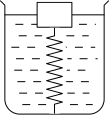
\includegraphics{figure/fig12.14}
    \caption{}
    \label{fig:12.14}
\end{wrapfigure}
水口流入下水道,在泄水口附近水流形成
涡旋状。在北半球,此涡旋为逆钟向的,为什么?
若在南半球,情况又怎样?

\question 一支盛水的圆桶,水中有一弹簧,
它的一端固定在桶底的中心,另一端系在
一浮标上,浮标浮在水面上开拉伸弹簧,
如图\ref{fig:12.14}所示。开始时,桶、水和浮标
都静止不动地放在一个高台子上,然后将支承桶的高台子突然撤
% 374.jpg
掉,使它们作为整体自由竖直下落,问弹簧和浮标将会发生什么
运动?

\end{questions}